%%%%%%%%%%%%%%%%%%%%%%%%%%%%%%%%%%%%%%%%%
% a0poster Portrait Poster
% LaTeX Template
% Version 1.0 (22/06/13)
%
% The a0poster class was created by:
% Gerlinde Kettl and Matthias Weiser (tex@kettl.de)
% 
% This template has been downloaded from:
% http://www.LaTeXTemplates.com
%
% License:
% CC BY-NC-SA 3.0 (http://creativecommons.org/licenses/by-nc-sa/3.0/)
%
%%%%%%%%%%%%%%%%%%%%%%%%%%%%%%%%%%%%%%%%%

%----------------------------------------------------------------------------------------
%	PACKAGES AND OTHER DOCUMENT CONFIGURATIONS
%----------------------------------------------------------------------------------------

\documentclass[a0,portrait]{a0poster}

\usepackage{multicol} % This is so we can have multiple columns of text side-by-side
\columnsep=100pt % This is the amount of white space between the columns in the poster
\columnseprule=3pt % This is the thickness of the black line between the columns in the poster

\usepackage[svgnames]{xcolor} % Specify colors by their 'svgnames', for a full list of all colors available see here: http://www.latextemplates.com/svgnames-colors

\usepackage{times} % Use the times font
%\usepackage{palatino} % Uncomment to use the Palatino font

\usepackage{graphicx} % Required for including images
\graphicspath{{../img/sketch/}{figures/}} % Location of the graphics files
\usepackage{booktabs} % Top and bottom rules for table
\usepackage[font=small,labelfont=bf]{caption} % Required for specifying captions to tables and figures
\usepackage{amsfonts, amsmath, amsthm, amssymb} % For math fonts, symbols and environments
\usepackage{wrapfig} % Allows wrapping text around tables and figures
\usepackage{epstopdf}
\epstopdfsetup{outdir=./}

\begin{document}

%----------------------------------------------------------------------------------------
%	POSTER HEADER 
%----------------------------------------------------------------------------------------

% The header is divided into two boxes:
% The first is 75% wide and houses the title, subtitle, names, university/organization and contact information
% The second is 25% wide and houses a logo for your university/organization or a photo of you
% The widths of these boxes can be easily edited to accommodate your content as you see fit

\begin{minipage}[b]{0.75\linewidth}
\veryHuge \textbf{Designing RNN for Explainability} \\ % Title
\large \textit{This work is part of master thesis.}\\[2cm] % Subtitle
\huge \textbf{Pattarawat Chormai} \\ [0.5cm]
\huge \textbf{Supervised by Dr. Gr\'{e}goire Montavon, Prof. Klaus-Robert M\"{u}ller} \\[0.5cm] % Author(s)
\huge Technical University Berlin, Department of Machine Learning \\[0.4cm] % University/organization
\Large \texttt{p.chormai@campus.tu-berlin.de} \\
\end{minipage}
%
\begin{minipage}[b]{0.25\linewidth}

\includegraphics[width=10cm]{tub-logo}\\
\end{minipage}

\vspace{1cm} % A bit of extra whitespace between the header and poster content

%----------------------------------------------------------------------------------------

\begin{multicols}{2} % This is how many columns your poster will be broken into, a portrait poster is generally split into 2 columns

%----------------------------------------------------------------------------------------
%	ABSTRACT
%----------------------------------------------------------------------------------------


%----------------------------------------------------------------------------------------
%	INTRODUCTION
%----------------------------------------------------------------------------------------

%\color{SaddleBrown} % SaddleBrown color for the introduction

\section*{Abstract}
Sed fringilla tempus hendrerit. Vestibulum ante ipsum primis in faucibus orci luctus et ultrices posuere cubilia Curae; Etiam ut elit sit amet metus lobortis consequat sit amet in libero. Lorem ipsum dolor sit amet, consectetur adipiscing elit. Phasellus vel sem magna. Nunc at convallis urna. isus ante. Pellentesque condimentum dui. Etiam sagittis purus non tellus tempor volutpat. Donec et dui non massa tristique adipiscing.

\section*{Introduction}

Aliquam non lacus dolor, \textit{a aliquam quam} \cite{Smith:2012qr}. Cum sociis natoque penatibus et magnis dis parturient montes, nascetur ridiculus mus. Nulla in nibh mauris. Donec vel ligula nisi, a lacinia arcu. Sed mi dui, malesuada vel consectetur et, egestas porta nisi. Sed eleifend pharetra dolor, et dapibus est vulputate eu. \textbf{Integer faucibus elementum felis vitae fringilla.} In hac habitasse platea dictumst. Duis tristique rutrum nisl, nec vulputate elit porta ut. Donec sodales sollicitudin turpis sed convallis. Etiam mauris ligula, blandit adipiscing condimentum eu, dapibus pellentesque risus.

\subsection*{Sensitivity Analysis}
\cite{SimonyanDeepConvolutionalNetworks2013}, an modified version \textbf{Guided Backprop}\cite{SpringenbergStrivingSimplicityAll2015}

%\subsection*{Guided Backprop}

\subsection*{Deep Taylor Decomposition}
\cite{MontavonExplainingnonlinearclassification2017}
\subsection*{Layer-Wise Relevance Propagation}
\cite{BachPixelWiseExplanationsNonLinear2015}
%----------------------------------------------------------------------------------------
%	OBJECTIVES
%----------------------------------------------------------------------------------------

\section*{Setting}
Dataset, problem training ... procedures ... 
\begin{center}\vspace{0.5cm}
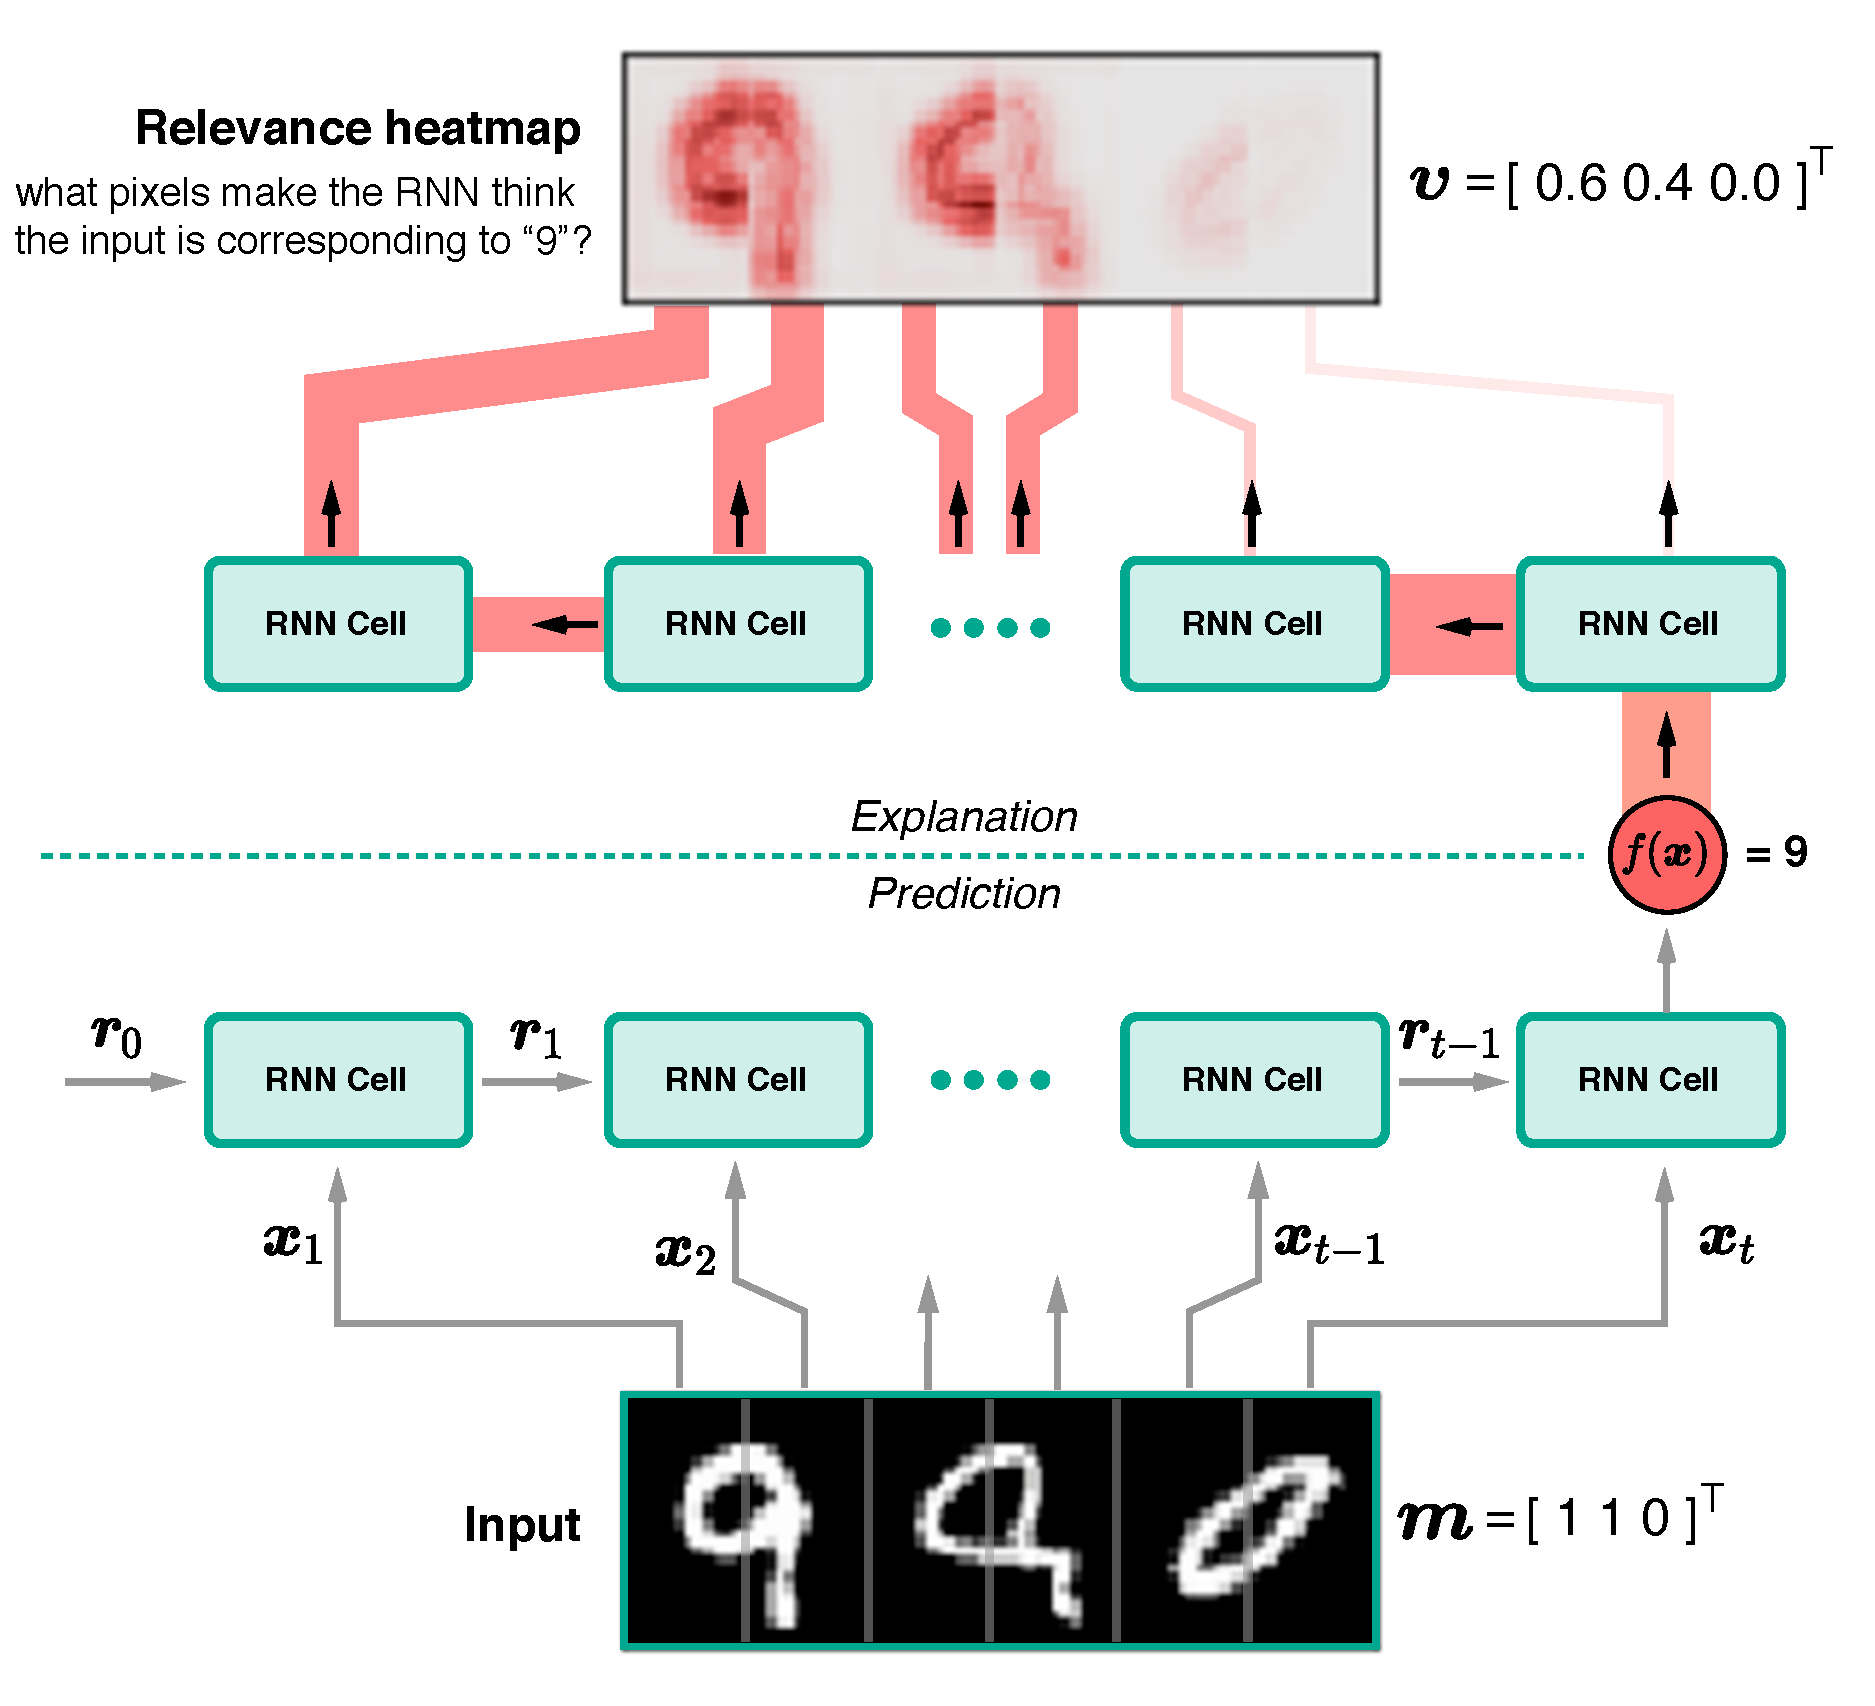
\includegraphics[width=0.6\linewidth]{artificial_problem_with_rel_poster}
\captionof{figure}{\color{Green} Figure caption}
\end{center}\vspace{0.5cm}

%----------------------------------------------------------------------------------------
%	MATERIALS AND METHODS
%----------------------------------------------------------------------------------------

Our quantitative evaluation is based on \textit{cosine similarity} between a binary vector $\boldsymbol{m} \in \mathbb{R}^3$, whose entry indicates whether the item belongs to the majority group, and a vector $\boldsymbol{v} \in \mathbb{R}^3$ representing percentage of relevance distributed to the corresponding  item.

$$
cos(\boldsymbol{m}, \boldsymbol{v}) = \frac{ \boldsymbol{m} \cdot\boldsymbol{v} }{||\boldsymbol{m}||||\boldsymbol{v}||}
$$


%\begin{center}\vspace{1cm}
%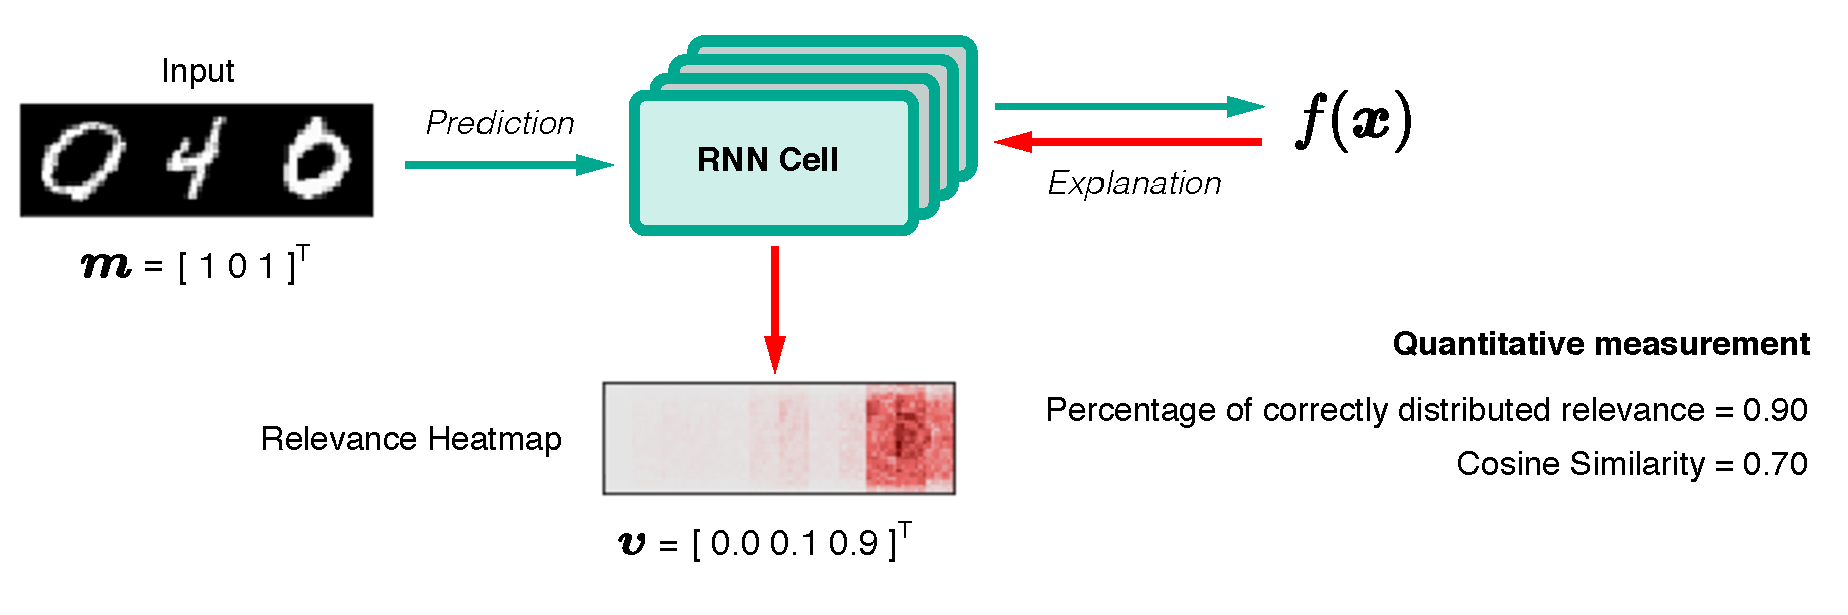
\includegraphics[width=0.8\linewidth]{quantitative_evaluation}
%\captionof{figure}{\color{Green} Figure caption}
%\end{center}\vspace{1cm}

%------------------------------------------------

\subsection*{Architectures}
Figure X shows RNN architectures considered in this study.

\begin{center}\vspace{0.5cm}
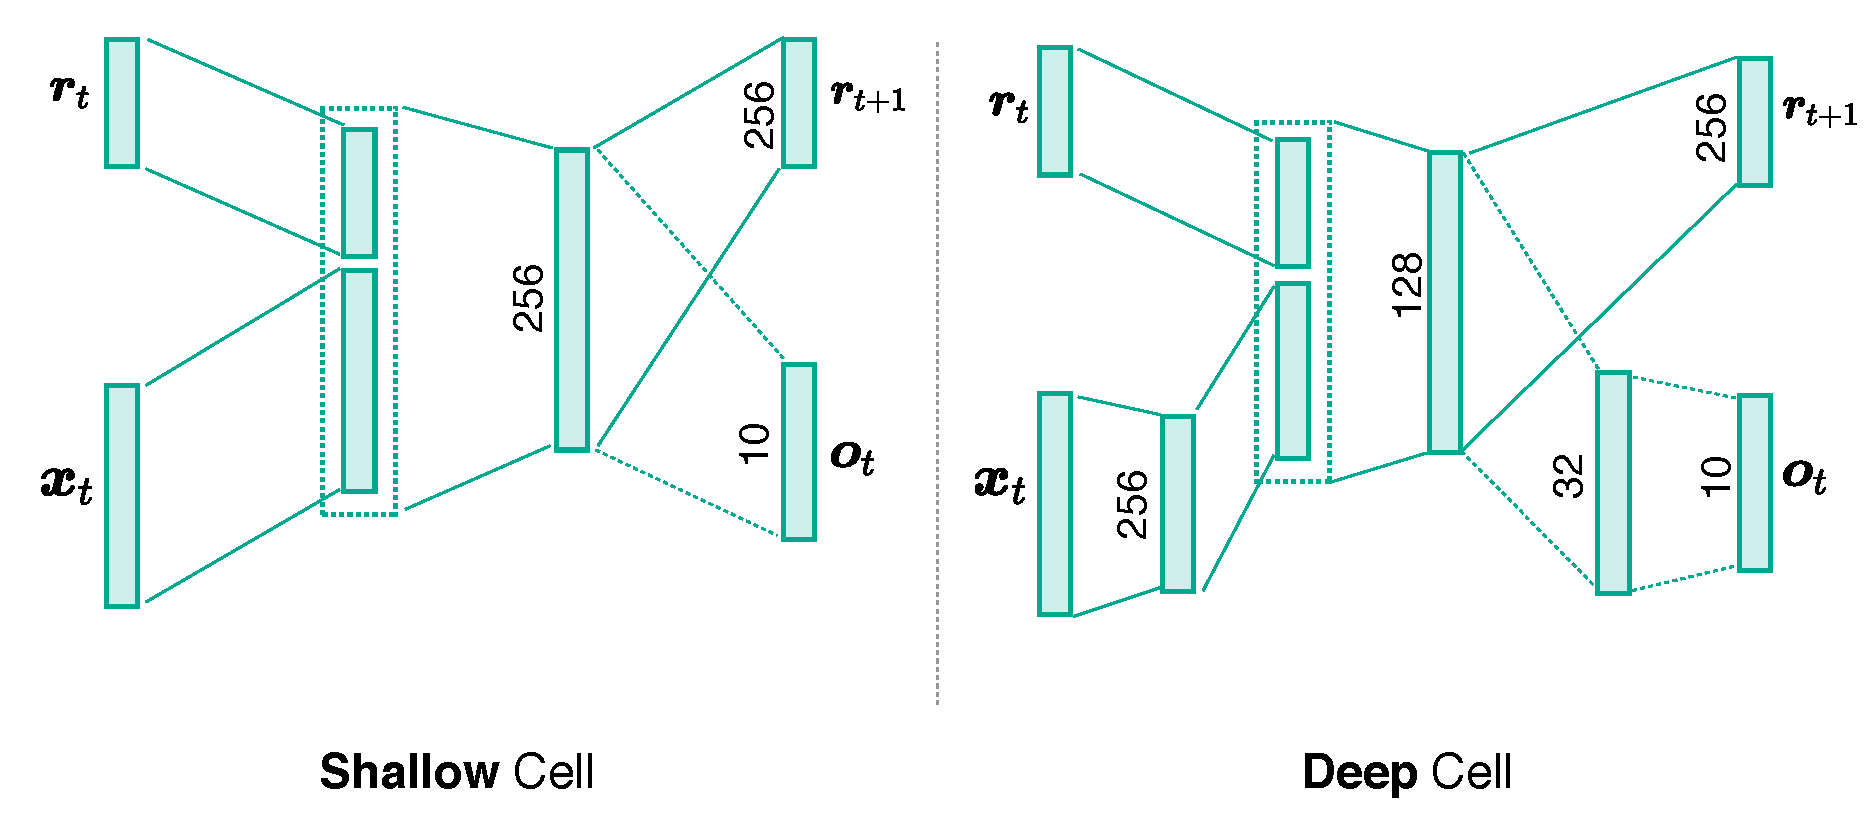
\includegraphics[width=0.7\linewidth]{architecture_with_number_neurons}
\captionof{figure}{\color{Green} Figure caption}
\end{center}\vspace{0.5cm}

%----------------------------------------------------------------------------------------
%	RESULTS 
%----------------------------------------------------------------------------------------

\section*{Results}

Donec faucibus purus at tortor egestas eu fermentum dolor facilisis. Maecenas tempor dui eu neque fringilla rutrum. Mauris \emph{lobortis} nisl accumsan. Aenean vitae risus ante.
Phasellus imperdiet, tortor vitae congue bibendum, felis enim sagittis lorem, et volutpat ante orci sagittis mi. Morbi rutrum laoreet semper. Morbi accumsan enim nec tortor consectetur non commodo nisi sollicitudin. Proin sollicitudin. Pellentesque eget orci eros. Fusce ultricies, tellus et pellentesque fringilla, ante massa luctus libero, quis tristique purus urna nec nibh.

\begin{center}\vspace{0.5cm}
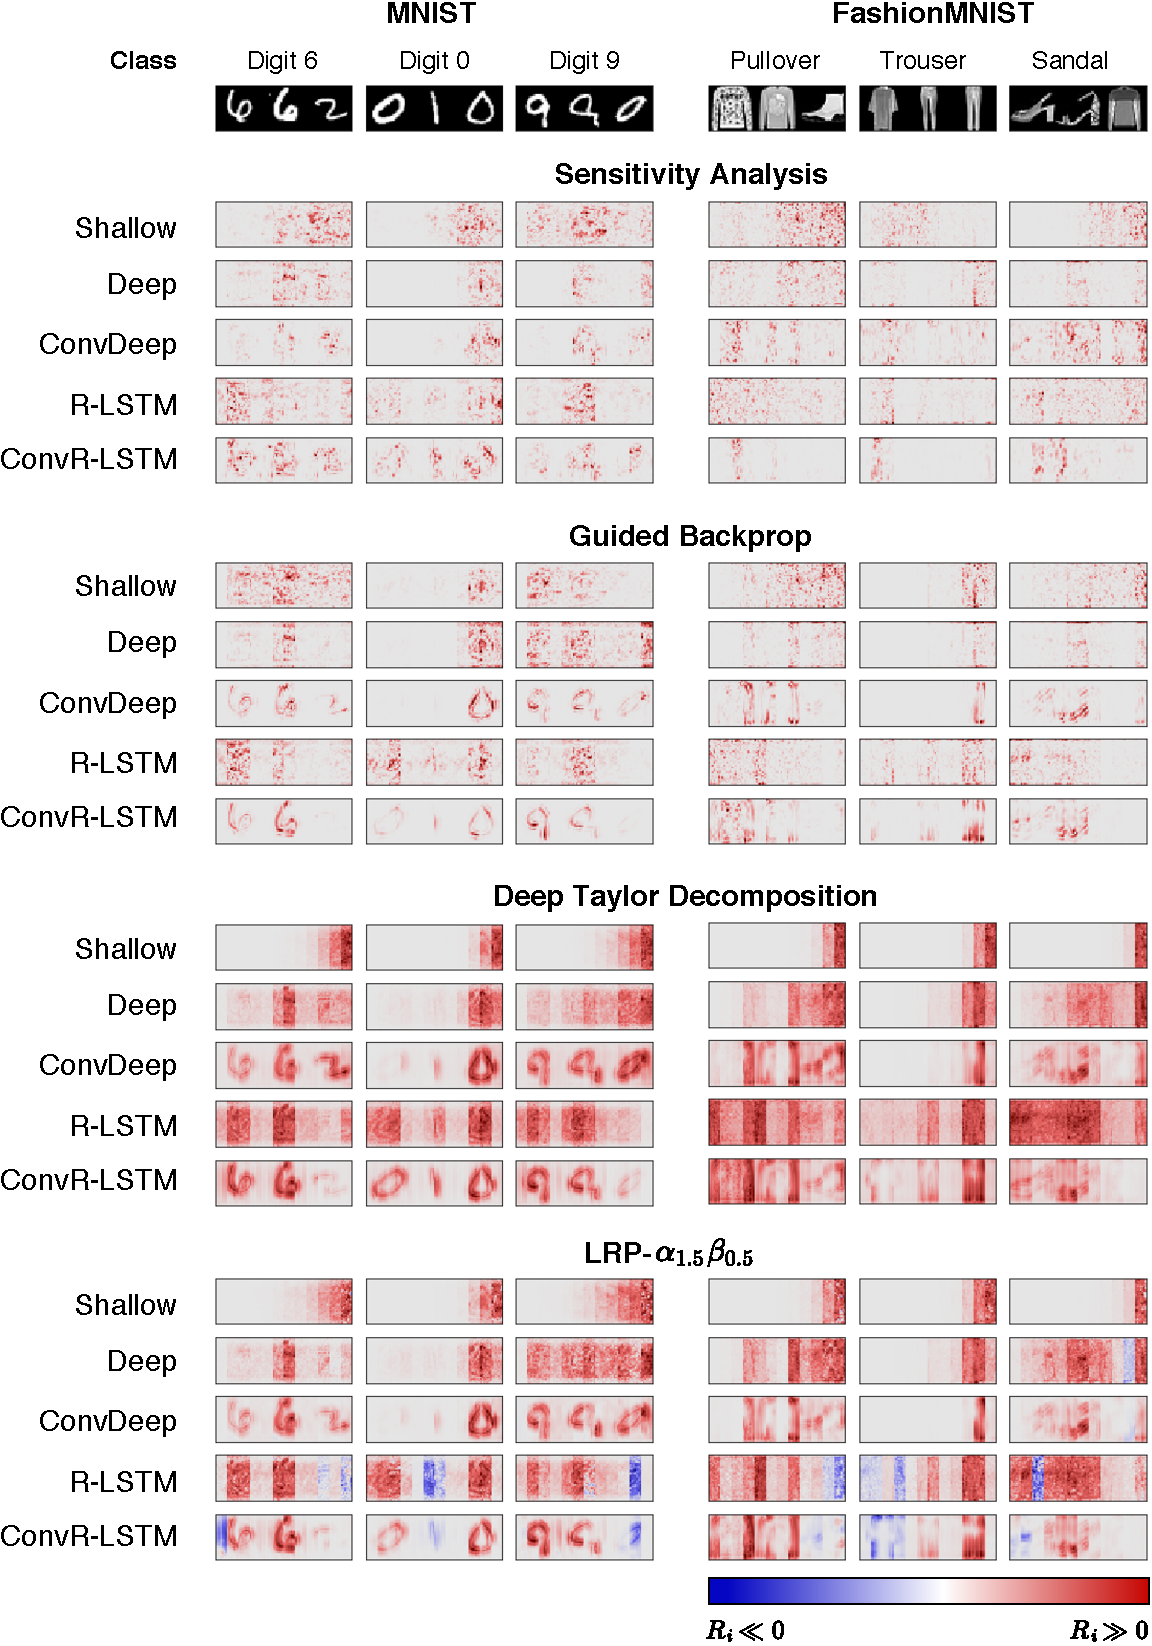
\includegraphics[width=0.8\linewidth]{heatmap_msc_poster}
%
\includegraphics[width=0.8\linewidth]{tub-logo}
\captionof{figure}{\color{Green} Figure caption}
\end{center}\vspace{0.5cm}

\begin{center}\vspace{0.5cm}
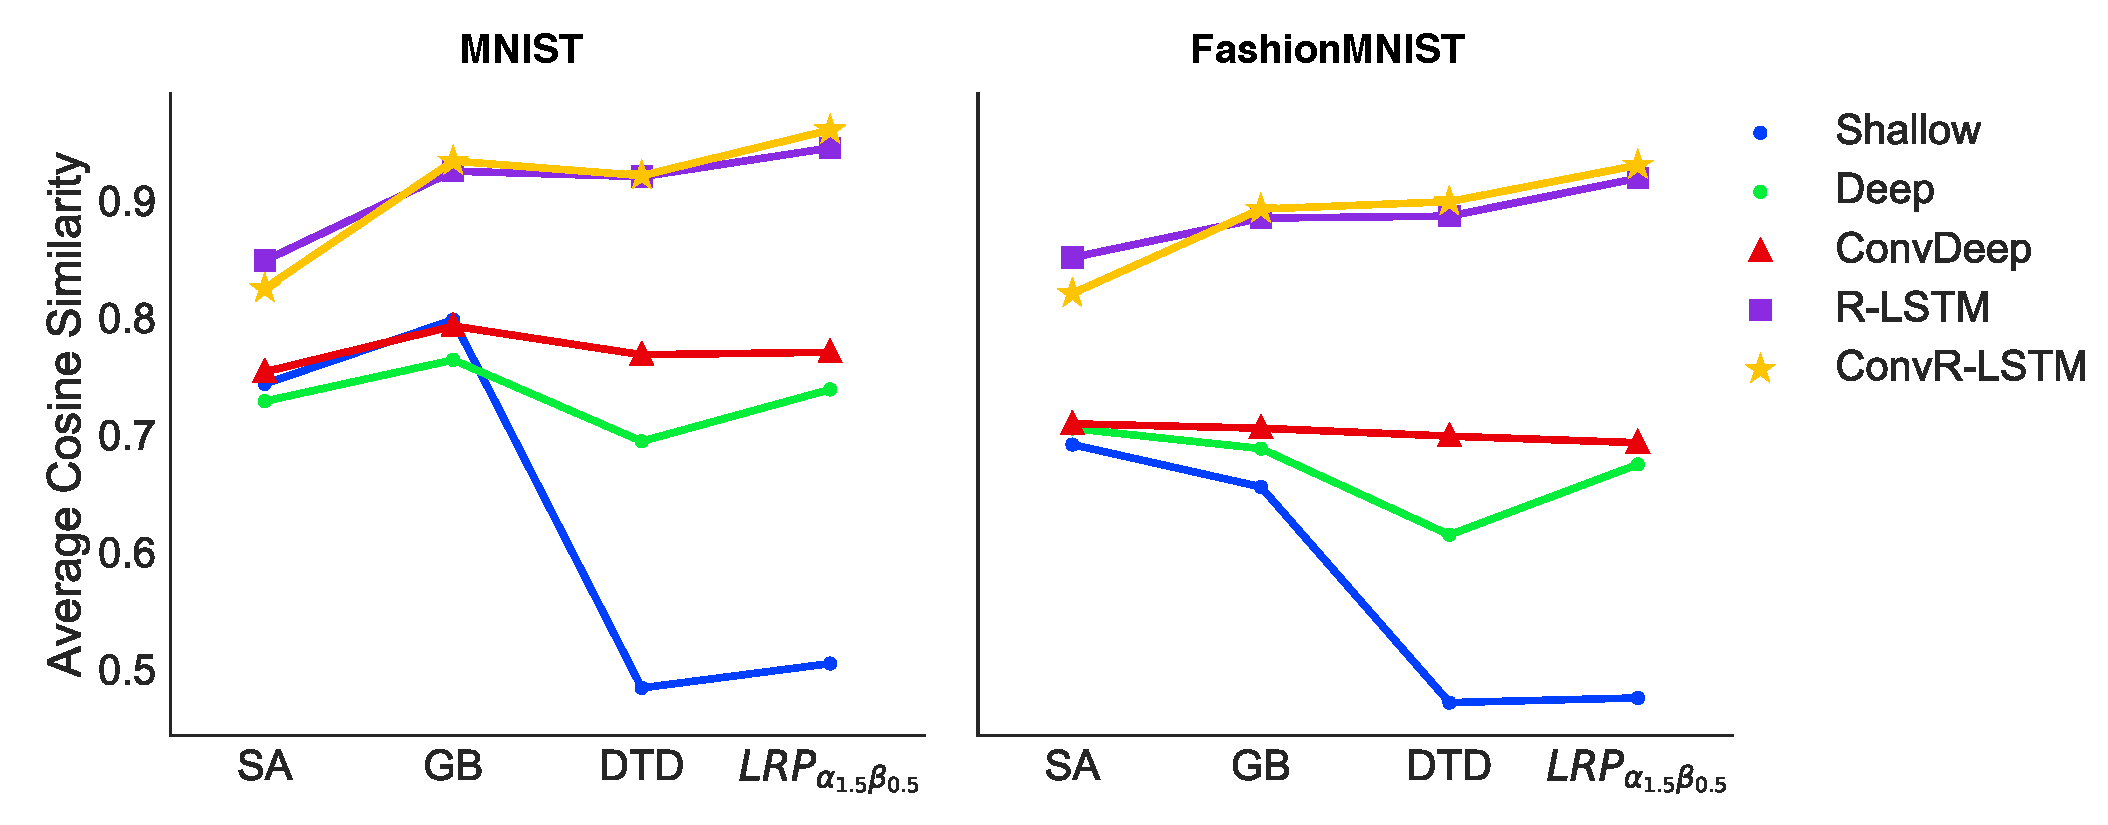
\includegraphics[width=0.7\linewidth]{rel_dist_maj_for_poster}
%
\includegraphics[width=0.8\linewidth]{tub-logo}
\captionof{figure}{\color{Green} Figure caption}
\end{center}\vspace{0.5cm}


%----------------------------------------------------------------------------------------
%	CONCLUSIONS
%----------------------------------------------------------------------------------------

\color{SaddleBrown} % SaddleBrown color for the conclusions to make them stand out

\section*{Conclusions}

\begin{itemize}
\item Pellentesque eget orci eros. Fusce ultricies, tellus et pellentesque fringilla, ante massa luctus libero, quis tristique purus urna nec nibh. Phasellus fermentum rutrum elementum. Nam quis justo lectus.
\item Vestibulum sem ante, hendrerit a gravida ac, blandit quis magna.
\item Donec sem metus, facilisis at condimentum eget, vehicula ut massa. Morbi consequat, diam sed convallis tincidunt, arcu nunc.
\item Nunc at convallis urna. isus ante. Pellentesque condimentum dui. Etiam sagittis purus non tellus tempor volutpat. Donec et dui non massa tristique adipiscing.
\end{itemize}

\color{DarkSlateGray} % Set the color back to DarkSlateGray for the rest of the content

%----------------------------------------------------------------------------------------
%	FORTHCOMING RESEARCH
%----------------------------------------------------------------------------------------

\section*{Future Work}

Vivamus molestie, risus tempor vehicula mattis, libero arcu volutpat purus, sed blandit sem nibh eget turpis. Maecenas rutrum dui blandit lorem vulputate gravida. Praesent venenatis mi vel lorem tempor at varius diam sagittis. Nam eu leo id turpis interdum luctus a sed augue. Nam tellus.

 %----------------------------------------------------------------------------------------
%	REFERENCES
%----------------------------------------------------------------------------------------

%\nocite{*} % Print all references regardless of whether they were cited in the poster or not
\bibliographystyle{abbrv} % Plain referencing style

\bibliography{../references.bib} % Use the example bibliography file sample.bib
%----------------------------------------------------------------------------------------
%	ACKNOWLEDGEMENTS
%----------------------------------------------------------------------------------------

\section*{Acknowledgements}

Etiam fermentum, arcu ut gravida fringilla, dolor arcu laoreet justo, ut imperdiet urna arcu a arcu. Donec nec ante a dui tempus consectetur. Cras nisi turpis, dapibus sit amet mattis sed, laoreet.

%----------------------------------------------------------------------------------------

\end{multicols}
\end{document}